\documentclass[a4paper,10pt]{article}
\usepackage[utf8]{inputenc}
\usepackage[T1]{fontenc}
\usepackage[english]{babel}
\usepackage[a4paper]{geometry}
\usepackage{graphicx}
\usepackage{float}


\title{Software Architectures\\ Assignment 5 : Software Visualizations}
\author{Arnaud Rosette, Simon Picard}

\begin{document}
\maketitle
\section{Exercise 1 : Analyzing the web portal application with an existing visualization}
\subsection{Chosen visualization}
As required by the assignment, we chose a predefined visualization of Moose. We decided to use the Blueprint complexity visualization because it highlights the complexity of a class, the cohesion inside a class, the coupling between different classes and the class hierarchy. So this visualization is able to show us the application architecture from a close perspective as well as a large perspective.
\begin{figure}[H]
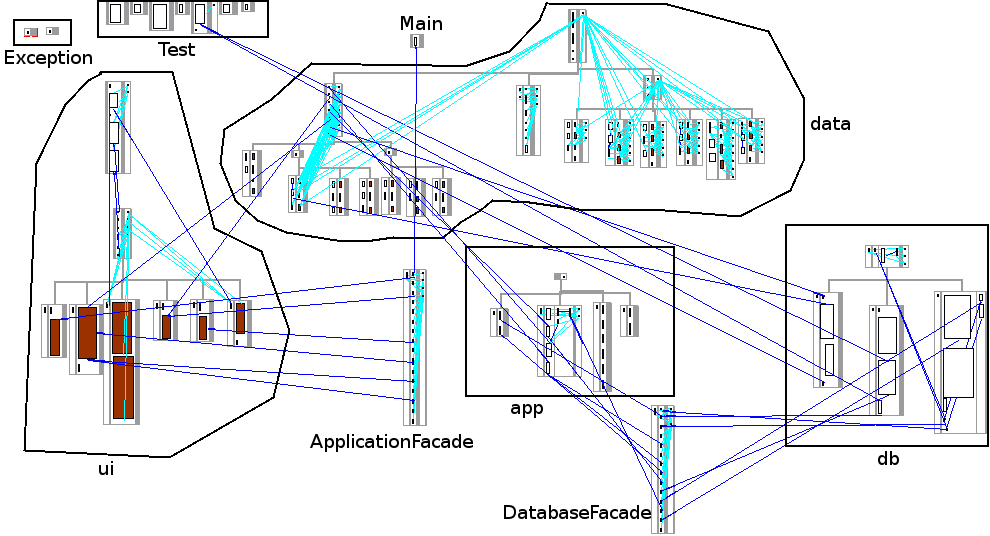
\includegraphics[width=\textwidth]{src/blueprint.png}
\centering
\caption{Class hierarchy Blueprint of the web\_portal application}
\end{figure}
\subsection{Lonely classes}
The visualization shows several classes that are isolated from the rest of application. They are classes which handle exceptions or classes managing test cases.\\
As we can see, the exception classes are only composed of one constructor. The coupling is very low between these classes and the rest of the application because the only thing that the other classes know about these classes is their constructor. It is a rather regular behavior for exception classes.\\
Most of test classes are essentially composed of one small  main method. It indicates that the test cases are poor in this application. Each test class only interacts with the class it needs to test. For example, TestRegularDatabase only interacts with RegularDatabase. It highlights the fact that the function of each test class is well defined. Some of the invocations are missing in this visualization for several test classes because each test class call at least one method of the class that it test.

\subsection{3-tier architecture}
The Blueprint visualization highlights the fact that the application is based on a layered architecture (3-tier architecture). We can see that each layer (ui, app and db) only interacts with the sub-layer through a facade. So the interface between each layer is clearly defined. We can notice that some invocations are missing from the ApplicationFacade to the app package.\\
The figure also shows that the two facades interact with concrete classes. The ApplicationFacade class uses concrete classes of the app package and DatabaseFacade uses concrete classes of the db package. DatabaseFacade interacts with the current implementation of the database layer which is a sql database. So coupling between different layers is rather low but coupling between a facade and classes inside the same package is quite high because facade uses directly concrete implementation. In order to address this issue, facades have to be independent from their layer implementation which means that facades have to talk to abstract classes instead of talking to concrete classes.

\subsection{Cohesion}
The graph exhibits a quite high cohesion inside classes. Indeed, most of the accesses are realized inside a class or between a sub-class and its parent class. The rest of the interactions between classes are invocations and their number is lower than that of accesses.

\subsection{Coupling}
The coupling between classes is relatively low thanks to the layered architecture but it can be improved because the coupling inside a package can be lower, especially between a facade and the classes in the same package. Facade classes have to interact with abstract classes in order to be able to switch from an implementation to another with few modifications in the facade class.

\section{Exercise 2 : Building your own visualization with Mondrian}
\end{document}
